\begin{frame}
\frametitle{Rotazioni: Asse x}
\begin{equation}
R_x(\theta) = 
\begin{bmatrix}
1 & 0 & 0 \\
0 & \mbox{cos}(\theta) & - \mbox{sen}(\theta)\\
0 & \mbox{sen}(\theta) & \mbox{cos}(\theta)
\end{bmatrix}
\end{equation}
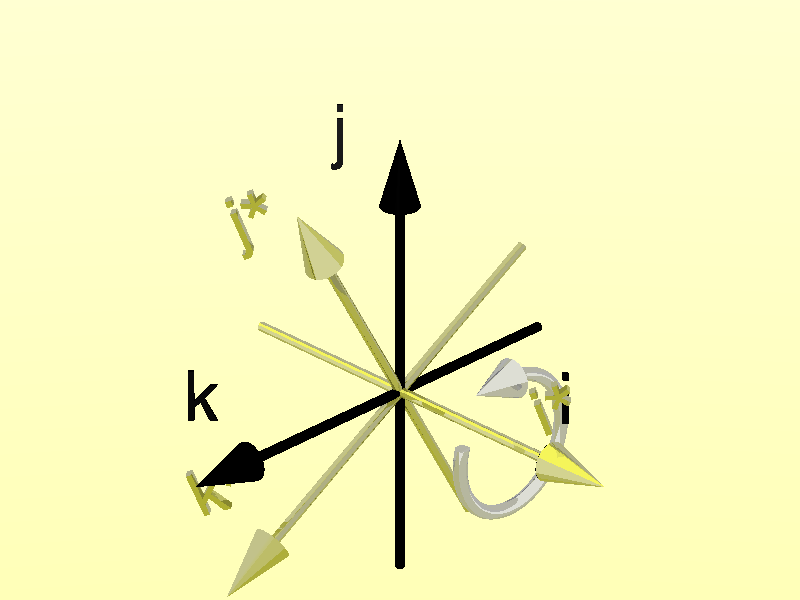
\includegraphics[width=0.7\textwidth]{\fig/rot_i_right.png}
\end{frame}
\begin{frame}
\frametitle{Rotazioni: Asse y}
\begin{equation}
R_y(\theta) = 
\begin{bmatrix}
\mbox{cos}(\theta) & 0 & \mbox{sen}(\theta)\\
0 & 1 & 0 \\
-\mbox{sen}(\theta)& 0 & \mbox{cos}(\theta)
\end{bmatrix}
\end{equation}
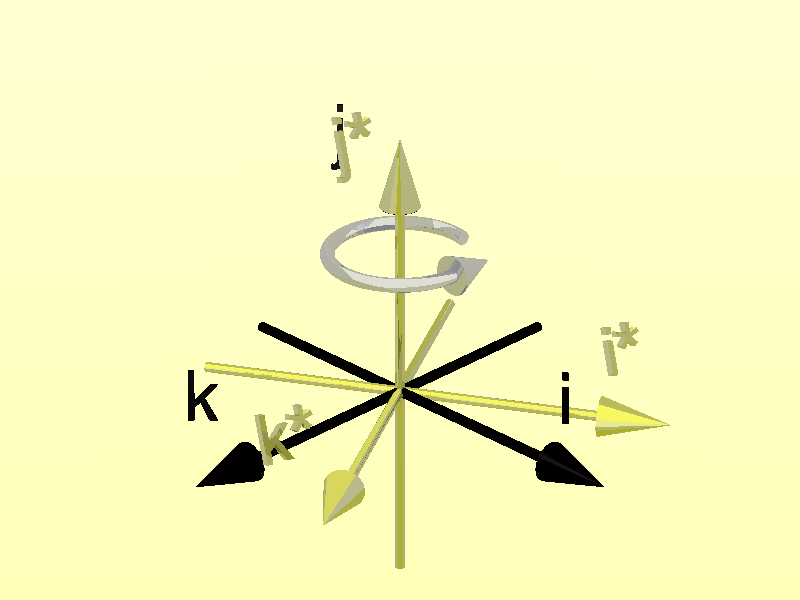
\includegraphics[width=0.7\textwidth]{\fig/rot_j_right.png}
\end{frame}
\begin{frame}
\frametitle{Rotazioni: Asse z}
\begin{equation}
R_z(\theta) = 
\begin{bmatrix}
\mbox{cos}(\theta) & - \mbox{sen}(\theta) & 0\\
\mbox{sen}(\theta) & \mbox{cos}(\theta)   & 0\\ 
0 & 0 & 1 
\end{bmatrix}
\end{equation}
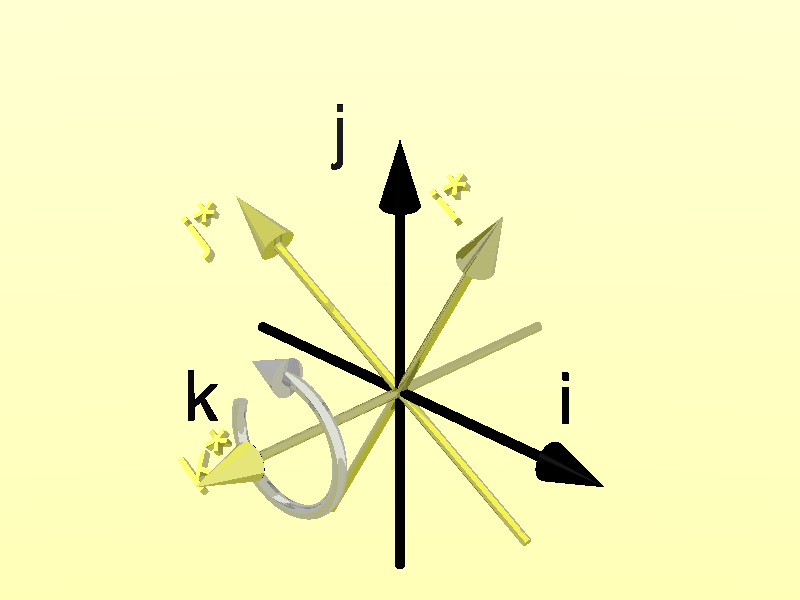
\includegraphics[width=0.7\textwidth]{\fig/rot_k_right.png}
\end{frame}
%
\begin{frame}
\frametitle{Tagli}
\begin{columns}
\begin{column}{0.48\textwidth}
Taglio in direzione x sulle facce con normale y:
\begin{equation}
T_{xy}=\begin{bmatrix}
    1 & k_x & 0\\
    0 & 1   & 0\\
    0 & 0   & 1
    \end{bmatrix}
\end{equation}
\end{column}
\begin{column}{0.48\textwidth}
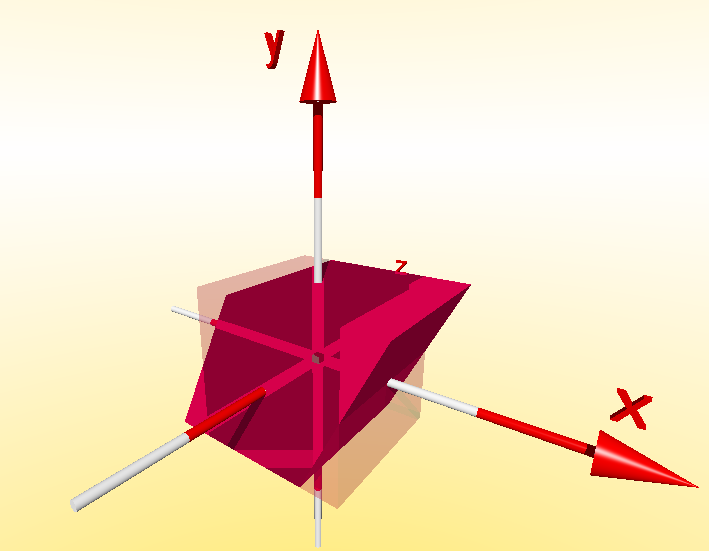
\includegraphics[width=0.8\textwidth]{\fig/cut_tx.png}
\end{column}
\end{columns}
%
\begin{columns}
\begin{column}{0.48\textwidth}
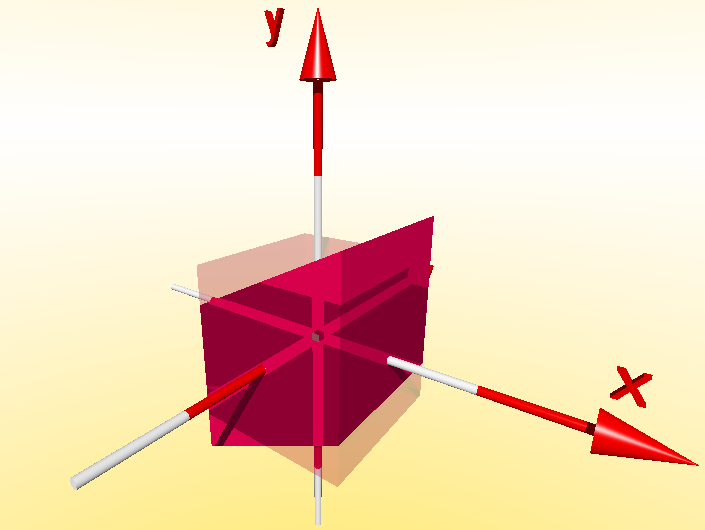
\includegraphics[width=0.8\textwidth]{\fig/cut_ty.png}
\end{column}
\begin{column}{0.48\textwidth}
Taglio in direzione y sulle facce con normale x:
\begin{equation}
T_{yx}=\begin{bmatrix}
    1   & 0 & 0\\
    k_y & 1 & 0\\
    0   & 0 & 1
    \end{bmatrix}
\end{equation}
\end{column}
\end{columns}
\end{frame}
%
\begin{frame}
\frametitle{Tagli[2]}
\begin{columns}
\begin{column}{0.48\textwidth}
Taglio in direzione z sulle facce con normale x:
\begin{equation}
T_{zx}=\begin{bmatrix}
    1 & 0 & 0\\
    0 & 1 & 0\\
    k_z & 0 & 1
    \end{bmatrix}
\end{equation}
\end{column}
\begin{column}{0.48\textwidth}
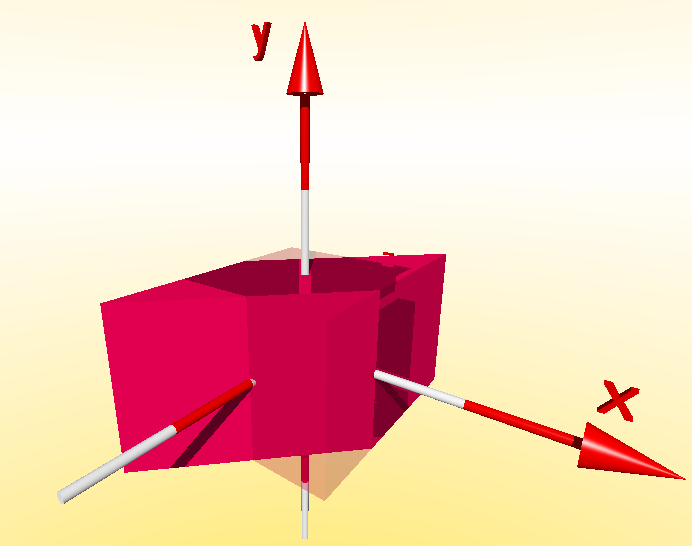
\includegraphics[width=0.8\textwidth]{\fig/cut_tz-x.png}
\end{column}
\end{columns}
%
%\begin{block}{}
\begin{columns}
\begin{column}{0.48\textwidth}
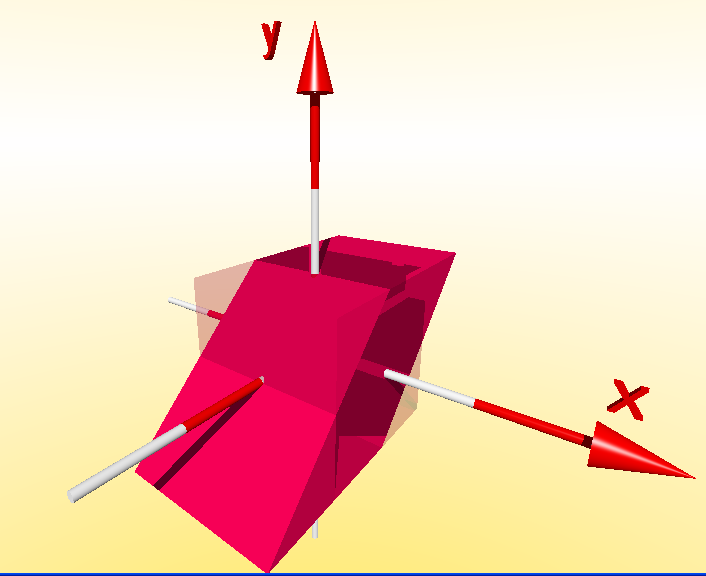
\includegraphics[width=0.8\textwidth]{\fig/cut_tz-y.png}
\end{column}
\begin{column}{0.48\textwidth}
Taglio in direzione z sulle facce con normale y:
\begin{equation}
T_{zy}=\begin{bmatrix}
    1 & 0 & 0\\
    0 & 1 & 0\\
    0 & k_z & 1
    \end{bmatrix}
\end{equation}
\end{column}
\end{columns}
%\end{block}
\end{frame}
%
\begin{frame}
\frametitle{Scalatura, Riflessione,Proiezione}
\begin{itemize}
\item Scalatura
\begin{equation}
S = \begin{bmatrix}
    S_x & 0 & 0\\
    0 & S_y & 0\\
    0 & 0 & S_z
    \end{bmatrix}
\end{equation}
\item Riflessione
\begin{equation}
F = \begin{bmatrix}
      1 & 0 & 0\\
      0 & 1 & 0\\
      0 & 0 & 1
    \end{bmatrix}
    -2~\begin{bmatrix}
    n_x \\
    n_y \\
    n_z
    \end{bmatrix} 
    ~\begin{bmatrix}
    n_x & n_y & n_z
    \end{bmatrix}
\end{equation}
\item Proiezione
\begin{equation}
 P = \begin{bmatrix}
      1 & 0 & 0\\
      0 & 1 & 0\\
      0 & 0 & 1
    \end{bmatrix}
    -\begin{bmatrix}
    n_x \\
    n_y \\
    n_z
    \end{bmatrix} 
    ~\begin{bmatrix}
    n_x & n_y & n_z
    \end{bmatrix}
\end{equation}
\end{itemize}
\end{frame}
%
\begin{frame}
\frametitle{Coordinate omogenee}
\begin{displaymath}
\begin{bmatrix}
a_{11} & a_{12} & a_{13} & t_1 \\
a_{21} & a_{22} & a_{23} & t_2 \\
a_{31} & a_{32} & a_{33} & t_3 \\
0      &    0   &  0     & 1 
\end{bmatrix}
~\begin{bmatrix}
x \\ y\\ z\\ 1
\end{bmatrix}
=  
\begin{bmatrix}
a_{11}x + a_{12}y + a_{13}z + t_1 \\
a_{21}x + a_{22}y + a_{23}z + t_2 \\
a_{31}x + a_{32}y + a_{33}z + t_3 \\
 1
\end{bmatrix}
\end{displaymath}
\end{frame}

